\section{A kereső fejlődése verzióról verzióra}\label{sec:versions}

A kereső minden jelentős módosítását robot-robot mérés követte: az új verzió (Improved searcher) a korábbi verzió (Old searcher) ellen játszott, a megnyitáskönyv véletlen kezdőállásaiból, színcserés párokban (\aref{sec:versioning}.~szakasz). \Aref{tab:versions}.~táblázat minden mérést felsorol a vizsgált változtatással együtt. A pontszám a győzelmek és a döntetlenek felének aránya, az Elo-különbség ebből a szokásos logisztikus modellel számolható:
\begin{equation}
	\Delta\mathrm{Elo} = -400 \log_{10}\!\left(\frac{1}{s}-1\right),
\end{equation}
ahol $s$ a pontszázalék.

\begin{table}[!ht]
	\scriptsize
	\centering
	\begin{tabularx}{\linewidth}{l l X r r r}
		\toprule
		Mérés & Dátum & Vizsgált változtatás & Gy/D/V & Pont & $\Delta$Elo \\
		\midrule
		v3 -- v2 & 04.24. & transzpozíciós tábla, delta-vágás a nyugalmi keresésben & 87/18/18 & 78,0\% & $+220$ $[+153;+306]$ \\
		v4 -- v3 & 04.25. & fail-soft vágások, gyökér a negamaxban & 379/360/261 & 55,9\% & $+41$ $[+20;+63]$ \\
		v5 -- v4 & 04.25. & gyilkos lépések & 391/366/243 & 57,4\% & $+52$ $[+30;+74]$ \\
		v6 -- v5 & 04.25. & történeti heurisztika & 260/251/189 & 55,1\% & $+35$ $[+10;+61]$ \\
		v7 -- v6 & 04.25. & PVS és késői lépések redukciója (LMR) & 61/41/9 & 73,4\% & $+177$ $[+109;+259]$ \\
		v8 -- v7 & 04.25. & null-lépés vágás & 322/545/133 & 59,5\% & $+66$ $[+45;+89]$ \\
		v8 -- v8 & 04.26. & ellenőrző mérés: azonos kód önmaga ellen & 28/51/27 & 50,5\% & $+3$ $[-64;+70]$ \\
		v9 -- v8 & 04.26. & fordított futility (statikus null-lépés), ,,javuló'' jelző & 102/124/40 & 61,7\% & $+82$ $[+41;+127]$ \\
		v10 -- v9 & 04.26. & futility vágás & 102/138/34 & 62,4\% & $+88$ $[+47;+132]$ \\
		v11 -- v10 & 04.26. & SEE-vágás a nyugalmi keresésben, SEE újraírása & 131/405/101 & 52,4\% & $+16$ $[-11;+44]$ \\
		v12 -- v11 & 04.27. & vesztes ütések és alulátváltozások hátrasorolása & 188/654/170 & 50,9\% & $+6$ $[-15;+28]$ \\
		v13 -- v12 & 04.27. & 4 elemes TT-klaszterek, előtöltés, időkezelés & 169/670/161 & 50,4\% & $+3$ $[-19;+24]$ \\
		v14 -- v13 & 04.28. & aspirációs ablak & 245/575/194 & 52,5\% & $+17$ $[-4;+39]$ \\
		v15 -- v14 & 04.28. & SEE-javítás, ismétlésfigyelés a táblában & 224/567/209 & 50,7\% & $+5$ $[-16;+27]$ \\
		v16 -- v15 & 04.28. & Lazy SMP többszálú keresés (csak 32 játszma) & 11/17/4 & 60,9\% & $+77$ $[-42;+218]$ \\
		v17 -- v15 & 05.02. & IID, LMR-módosítók, gyökérlépés-rendezés, lusta lépésválasztás & 160/362/153 & 50,5\% & $+4$ $[-23;+30]$ \\
		v18 -- v17 & 05.30. & történeti ,,gravitáció'' és büntetés, history-tag az LMR-ben & 220/670/137 & 54,0\% & $+28$ $[+7;+50]$ \\
		v23 -- today & 10.12. & zármentes TT, TT a nyugalmi keresésben, IIR, teljes fail-soft, új aspiráció & 360/605/35 & 66,2\% & $+117$ $[+95;+140]$ \\
		\bottomrule
	\end{tabularx}
	\caption{Az összes verziómérés (2026). Gy/D/V: az új verzió győzelmei, döntetlenjei és vereségei.}
	\label{tab:versions}
\end{table}

\begin{figure}[!ht]
	\centering
	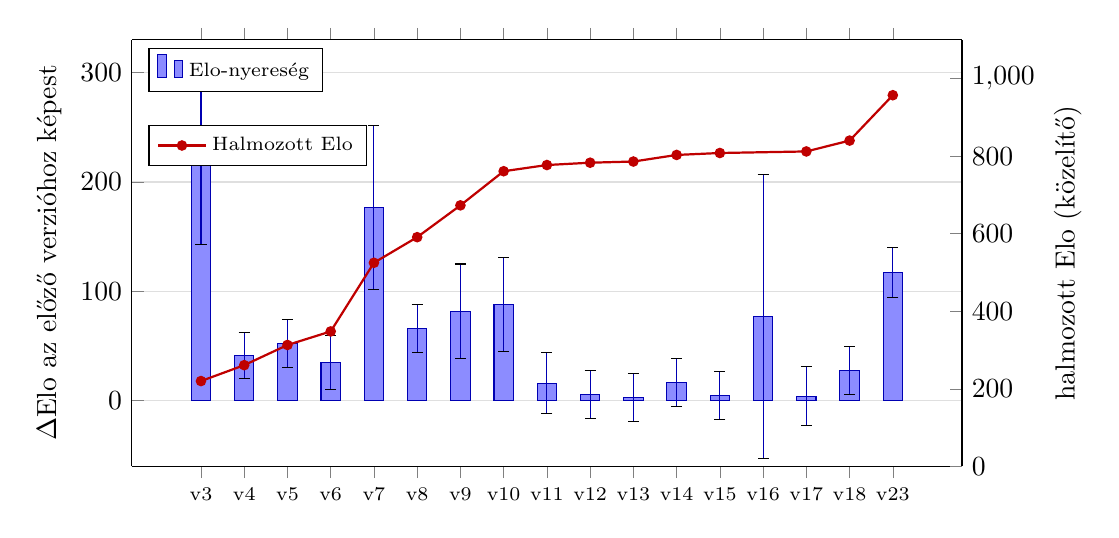
\begin{tikzpicture}
		\begin{axis}[
			width=\linewidth, height=7cm,
			ybar, bar width=7pt,
			ylabel={$\Delta$Elo az előző verzióhoz képest},
			symbolic x coords={v3,v4,v5,v6,v7,v8,v9,v10,v11,v12,v13,v14,v15,v16,v17,v18,v23},
			xtick=data, x tick label style={font=\scriptsize},
			ymin=-60, ymax=330,
			ymajorgrids, grid style={gray!25},
			axis y line*=left,
			legend style={at={(0.02,0.98)}, anchor=north west, font=\scriptsize},
		]
			\addplot[fill=blue!45, draw=blue!70!black, error bars/.cd, y dir=both, y explicit]
				coordinates {
					(v3,220) +- (0,77) (v4,41) +- (0,21) (v5,52) +- (0,22) (v6,35) +- (0,25)
					(v7,177) +- (0,75) (v8,66) +- (0,22) (v9,82) +- (0,43) (v10,88) +- (0,43)
					(v11,16) +- (0,28) (v12,6) +- (0,22) (v13,3) +- (0,22) (v14,17) +- (0,22)
					(v15,5) +- (0,22) (v16,77) +- (0,130) (v17,4) +- (0,27) (v18,28) +- (0,22) (v23,117) +- (0,23)
				};
			\addlegendentry{Elo-nyereség}
		\end{axis}
		\begin{axis}[
			width=\linewidth, height=7cm,
			symbolic x coords={v3,v4,v5,v6,v7,v8,v9,v10,v11,v12,v13,v14,v15,v16,v17,v18,v23},
			xtick=\empty, axis x line=none,
			axis y line*=right, ymin=0, ymax=1100,
			ylabel={halmozott Elo (közelítő)},
			legend style={at={(0.02,0.80)}, anchor=north west, font=\scriptsize},
		]
			\addplot[red!75!black, thick, mark=*, mark size=1.5pt]
				coordinates {
					(v3,220) (v4,261) (v5,313) (v6,348) (v7,525) (v8,591) (v9,673) (v10,761)
					(v11,777) (v12,783) (v13,786) (v14,803) (v15,808) (v17,812) (v18,840) (v23,957)
				};
			\addlegendentry{Halmozott Elo}
		\end{axis}
	\end{tikzpicture}
	\caption{Az egyes verziók erősödése az előző verzióhoz képest (oszlopok) és az ebből halmozott, közelítő Elo-nyereség (vonal). A v16 mérés csak 32 játszmából áll, ezért a halmozott értékbe nem számít bele.}
	\label{fig:versions}
\end{figure}

\Aref{fig:versions}.~ábra jól mutatja a fejlesztés két szakaszát. Az első napokban az alapvető technikák (TT, PVS és LMR, null-lépés, futility-vágások) egyenként is 35--220 Elo-pontot hoztak. A v11--v17 közötti módosítások már csak néhány Elo-pontos, a mérési hibán belüli javulást adtak; ezek nagy része tisztán sebesség- vagy robusztussági javítás volt (pl. TT-klaszterek, SEE-hibák javítása), amelyek a játékerőn rövid időkontrollal alig látszanak. A legnagyobb késői ugrást a v23 hozta: a zármentes transzpozíciós tábla, a nyugalmi keresésben is használt TT és az IIR együtt $+117$ Elo-pontot ért a közvetlen előd ellen. A közelítő halmozott nyereség a v2-től a v23-ig mintegy 950 Elo-pont; ez csak tájékoztató érték, mert a láncban a mérések nem mindig közvetlenül egymást követő verziók között történtek.

A legkorábbi, még a felülettel együtt fejlesztett keresőt (a v21 és v22 archív verziót, 2026.~április~21.) a fenti sorozat nem tartalmazza: ezeket csak néhány tucat, illetve négy próbajátszmával mértem, és a v1-ben a keresőt tudatosan egy minimális magról, lépésenként újraépítettem, hogy minden technika hatása külön mérhető legyen.
